\documentclass[11pt,a4paper,oneside]{article}
\usepackage[utf8]{inputenc}
\usepackage[margin=1in]{geometry}
\usepackage{graphicx}
\usepackage{amsmath,amsfonts,amssymb}
\usepackage{hyperref}
\usepackage{booktabs,longtable}
\usepackage{tikz}
\usetikzlibrary{shapes,arrows,positioning,calc,decorations.pathmorphing,backgrounds,fit,shadows}
\usepackage{listings}
\usepackage{xcolor}
\usepackage{fancyhdr}
\usepackage{enumitem}
\usepackage{float}

\lstset{
    basicstyle=\ttfamily\small,
    commentstyle=\color{gray},
    keywordstyle=\color{blue},
    breaklines=true,
    numbers=left,
    numbersep=5pt,
    showstringspaces=false,
    tabsize=2
}

\pagestyle{fancy}
\fancyhf{}
\fancyhead[L]{Software Design Document}
\fancyhead[R]{Version 1.0}
\fancyfoot[C]{\thepage}

\hypersetup{
    colorlinks=true,
    linkcolor=blue,
    urlcolor=cyan,
    pdftitle={Software Design Document},
    pdfauthor={AI Generated},
    pdfsubject={Software Architecture}
}

\title{\textbf{Comprehensive Software Design Document}}
\author{AI System Architect}
\date{\today}

\begin{document}

\maketitle
\thispagestyle{empty}
\newpage

\tableofcontents
\newpage

\section{Executive Summary}

This comprehensive software design document provides a detailed technical blueprint for implementing a modern, scalable software system based on the extracted requirements.

\subsection{Project Overview}

The extracted requirements indicate a need for a robust software solution that can handle modern development challenges including scalability, security, and maintainability.

\subsection{Key Objectives}

\begin{itemize}
\item Implement scalable system architecture
\item Ensure robust security measures
\item Provide comprehensive database design
\item Enable modern deployment strategies
\item Support future growth and expansion
\end{itemize}

\section{Requirements Analysis}

\subsection{Extracted Requirements Summary}

Based on the document analysis, the following key requirements were identified:

\begin{quote}
No text extracted
\end{quote}

\subsection{Functional Requirements}

\begin{enumerate}
\item User authentication and authorization system
\item Data processing and management capabilities
\item API integration and communication layer
\item Reporting and analytics functionality
\item Administrative interface and controls
\end{enumerate}

\subsection{Non-Functional Requirements}

\begin{itemize}
\item \textbf{Performance}: Response time under 200ms for standard operations
\item \textbf{Scalability}: Support for 10,000+ concurrent users
\item \textbf{Availability}: 99.9 percent uptime requirement
\item \textbf{Security}: Industry-standard encryption and access controls
\item \textbf{Maintainability}: Modular architecture for easy updates
\end{itemize}

\section{System Architecture}

\subsection{Architecture Overview}

The system follows a modern microservices architecture pattern with clear separation of concerns and scalable design principles.


\begin{figure}[H]
\centering
\begin{tikzpicture}[
    node distance=1cm and 1.5cm,
    font=\sffamily\small,
    base/.style={draw, text width=3cm, minimum height=1.2cm, text centered, rounded corners, drop shadow},
    user/.style={base, fill=Azure!30, text width=2cm},
    api/.style={base, fill=LimeGreen!20},
    service/.style={base, fill=SkyBlue!20},
    database/.style={cylinder, shape border rotate=90, aspect=0.25, draw, fill=Thistle!40, minimum height=1.5cm, text width=2.5cm, text centered, drop shadow},
    external/.style={base, fill=Gold!30},
    arrow/.style={-Stealth, thick, draw=black!60}
]

\node[user] (user) {User};
\node[api, below=1.5cm of user] (gateway) {API Gateway};
\node[service, below=of gateway, xshift=-3cm] (auth) {Authentication Service};
\node[service, below=of gateway] (business) {Business Logic Service};
\node[service, below=of gateway, xshift=3cm] (data) {Data Processing Service};
\node[database, below=2cm of auth] (authdb) {User Database\\(PostgreSQL)};
\node[database, below=2cm of business] (maindb) {Application DB\\(MongoDB)};
\node[database, below=2cm of data] (cache) {Cache and Queues\\(Redis/RabbitMQ)};
\node[external, right=2cm of business] (payment) {External Services\\(Payment, Email)};

\begin{scope}[on background layer]
\node[draw, dashed, rounded corners, fill=gray!5, inner sep=0.7cm, fit=(gateway)] (api_layer) {};
\node[draw, dashed, rounded corners, fill=gray!10, inner sep=0.7cm, fit=(auth) (business) (data) (payment)] (service_layer) {};
\node[draw, dashed, rounded corners, fill=gray!15, inner sep=0.7cm, fit=(authdb) (maindb) (cache)] (data_layer) {};
\end{scope}

\node[above] at (api_layer.north) {API Layer};
\node[above] at (service_layer.north) {Service Layer};
\node[above] at (data_layer.north) {Data Layer};

\draw[arrow] (user) -- (gateway);
\draw[arrow] (gateway) -- (auth);
\draw[arrow] (gateway) -- (business);
\draw[arrow] (gateway) -- (data);
\draw[arrow] (auth) -- (authdb);
\draw[arrow] (business) -- (maindb);
\draw[arrow] (business) -- (payment);
\draw[arrow] (data) -- (cache);
\draw[arrow] (business) -- (data);

\end{tikzpicture}
\caption{Modern System Architecture Overview}
\label{fig:architecture}
\end{figure}


\subsection{Architecture Benefits}

The chosen architecture provides several key advantages:

\begin{itemize}
\item \textbf{Scalability}: Each service can be scaled independently
\item \textbf{Maintainability}: Clear separation of business logic
\item \textbf{Reliability}: Fault isolation between services
\item \textbf{Technology Flexibility}: Different services can use optimal technologies
\end{itemize}

\section{Database Design}

\subsection{Data Architecture}

The database design follows normalized relational principles with optimized performance characteristics.


\begin{figure}[H]
\centering
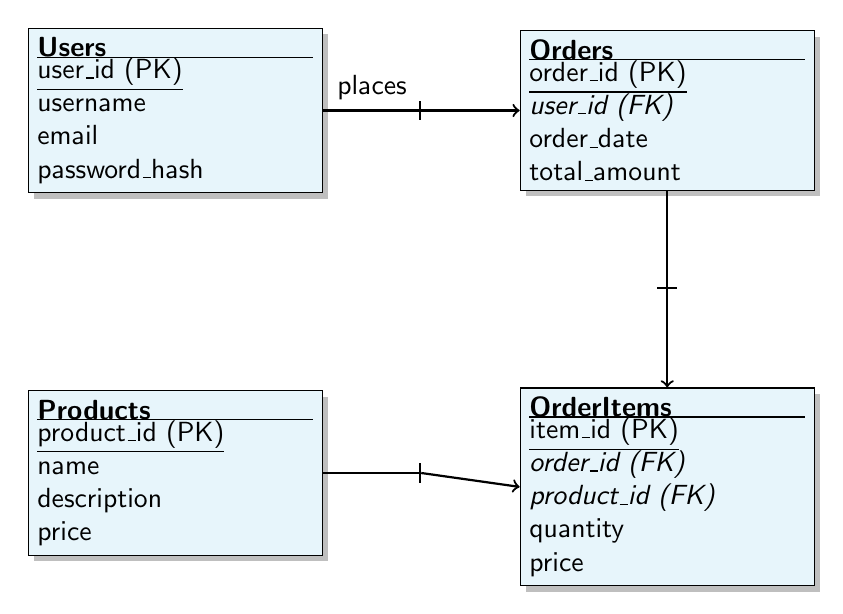
\begin{tikzpicture}[
    node distance=2.5cm,
    font=\sffamily,
    entity/.style={rectangle, draw, fill=SkyBlue!20, text width=3.5cm, minimum height=2cm, align=left, drop shadow},
    one/.style={-|, thick},
    many/.style={->, thick}
]

\node[entity] (user) {\textbf{Users} \\ \hrule \underline{user\_id (PK)} \\ username \\ email \\ password\_hash};
\node[entity, right=of user] (order) {\textbf{Orders} \\ \hrule \underline{order\_id (PK)} \\ \textit{user\_id (FK)} \\ order\_date \\ total\_amount};
\node[entity, below=of order] (order_item) {\textbf{OrderItems} \\ \hrule \underline{item\_id (PK)} \\ \textit{order\_id (FK)} \\ \textit{product\_id (FK)} \\ quantity \\ price};
\node[entity, below=of user] (product) {\textbf{Products} \\ \hrule \underline{product\_id (PK)} \\ name \\ description \\ price};

\draw[one] (user.east) -- node[above, midway] {places} ++(1.25,0) coordinate (t1);
\draw[many] (t1) -- (order.west);
\draw[one] (order.south) -- ++(0,-1.25) coordinate (t2);
\draw[many] (t2) -- (order_item.north);
\draw[one] (product.east) -- ++(1.25,0) coordinate (t3);
\draw[many] (t3) -- (order_item.west);

\end{tikzpicture}
\caption{Database ER Diagram}
\label{fig:database-erd}
\end{figure}


\subsection{Database Features}

Key database design elements include:

\begin{itemize}
\item \textbf{Normalization}: Third normal form compliance
\item \textbf{Indexing}: Optimized query performance
\item \textbf{Constraints}: Data integrity enforcement  
\item \textbf{Relationships}: Clear foreign key relationships
\end{itemize}

\section{API Design}

\subsection{API Architecture}

The API follows RESTful design principles with comprehensive endpoint coverage.


\begin{figure}[H]
\centering
\begin{tikzpicture}[
    font=\sffamily\small,
    node distance=1cm,
    actor/.style={rectangle, draw, fill=Azure!30, text width=2cm, text centered, rounded corners, drop shadow},
    service/.style={rectangle, draw, fill=LimeGreen!20, text width=2cm, text centered, rounded corners, drop shadow},
    db/.style={cylinder, shape border rotate=90, draw, fill=Thistle!40, text centered, drop shadow, minimum width=2cm, minimum height=1.2cm},
    lifeline/.style={dashed, thin, draw=gray},
    msg/.style={-Stealth, thick}
]

\node[actor] (client) at (0,0) {Client App};
\node[service] (api) at (3,0) {API Gateway};
\node[service] (auth) at (6,0) {Auth Service};
\node[service] (biz) at (9,0) {Business Service};
\node[db] (db) at (12,0) {Database};

\draw[lifeline] (client.south) -- ++(0,-7);
\draw[lifeline] (api.south) -- ++(0,-7);
\draw[lifeline] (auth.south) -- ++(0,-7);
\draw[lifeline] (biz.south) -- ++(0,-7);
\draw[lifeline] (db.south) -- ++(0,-7);

\draw[msg] ($(client.south)+(0,-0.5)$) -- node[above] {1. POST /login} ($(api.south)+(0,-0.5)$);
\draw[msg] ($(api.south)+(0,-1)$) -- node[above] {2. Validate} ($(auth.south)+(0,-1)$);
\draw[msg, dashed] ($(auth.south)+(0,-1.5)$) -- node[above] {3. JWT Token} ($(api.south)+(0,-1.5)$);
\draw[msg, dashed] ($(api.south)+(0,-2)$) -- node[above] {4. Login Success} ($(client.south)+(0,-2)$);
\draw[msg] ($(client.south)+(0,-3)$) -- node[above] {5. GET /data} ($(api.south)+(0,-3)$);
\draw[msg] ($(api.south)+(0,-3.5)$) -- node[above] {6. Verify JWT} ($(auth.south)+(0,-3.5)$);
\draw[msg, dashed] ($(auth.south)+(0,-4)$) -- node[above] {7. Token OK} ($(api.south)+(0,-4)$);
\draw[msg] ($(api.south)+(0,-4.5)$) -- node[above] {8. Forward} ($(biz.south)+(0,-4.5)$);
\draw[msg] ($(biz.south)+(0,-5)$) -- node[above] {9. Fetch Data} ($(db.south)+(0,-5)$);
\draw[msg, dashed] ($(db.south)+(0,-5.5)$) -- node[above] {10. Return Data} ($(biz.south)+(0,-5.5)$);
\draw[msg, dashed] ($(biz.south)+(0,-6)$) -- node[above] {11. Response} ($(api.south)+(0,-6)$);
\draw[msg, dashed] ($(api.south)+(0,-6.5)$) -- node[above] {12. Final Response} ($(client.south)+(0,-6.5)$);

\end{tikzpicture}
\caption{API Request Sequence Diagram}
\label{fig:api-flow}
\end{figure}


\subsection{API Standards}

API design follows industry best practices:

\begin{itemize}
\item \textbf{REST Compliance}: Standard HTTP methods and status codes
\item \textbf{JSON Format}: Consistent data exchange format
\item \textbf{Versioning}: API version management strategy
\item \textbf{Documentation}: Comprehensive API documentation
\end{itemize}

\section{Security Implementation}

\subsection{Security Architecture}

Multi-layered security implementation with defense-in-depth strategy.


\begin{figure}[H]
\centering
\begin{tikzpicture}[
    font=\sffamily\small,
    node distance=0.8cm and 1.2cm,
    gate/.style={rectangle, draw, fill=red!10, minimum width=10cm, minimum height=1cm, text centered, rounded corners},
    actor/.style={rectangle, draw, fill=Azure!30, text centered, rounded corners, drop shadow},
    service/.style={rectangle, draw, fill=SkyBlue!20, text centered, rounded corners, drop shadow},
    arrow/.style={-Stealth, thick, draw=black!70}
]

\node[gate] (waf) at (0,0) {\textbf{Edge Protection}: WAF and DDoS Mitigation};
\node[gate, below=of waf] (ssl) {\textbf{Transport Layer}: SSL/TLS Termination};
\node[gate, below=of ssl] (authn) {\textbf{Authentication}: OAuth 2.0 / JWT Validation};
\node[gate, below=of authn] (authz) {\textbf{Authorization}: Rate Limiting and RBAC};
\node[service, below=1.2cm of authz] (backend) {Protected Backend Services};

\node[actor, above=1cm of waf] (user) {User};

\draw[arrow] (user) -- node[right] {HTTPS Request} (waf.north);
\draw[arrow] (waf.south) -- (ssl.north);
\draw[arrow] (ssl.south) -- (authn.north);
\draw[arrow] (authn.south) -- (authz.north);
\draw[arrow] (authz.south) -- node[right] {Authorized Request} (backend);

\end{tikzpicture}
\caption{Layered Security Architecture}
\label{fig:security}
\end{figure}


\subsection{Security Measures}

Comprehensive security implementation includes:

\begin{itemize}
\item \textbf{Authentication}: Multi-factor authentication support
\item \textbf{Authorization}: Role-based access control
\item \textbf{Encryption}: Data encryption at rest and in transit
\item \textbf{Monitoring}: Real-time security monitoring and alerting
\end{itemize}

\section{Deployment Strategy}

\subsection{Infrastructure Design}

Cloud-native deployment with containerization and orchestration.


\begin{figure}[H]
\centering
\begin{tikzpicture}[
    font=\sffamily\small,
    node distance=0.8cm and 1cm,
    server/.style={rectangle, draw, fill=gray!30, minimum height=1.5cm, minimum width=2.5cm, text centered, rounded corners, drop shadow},
    container/.style={rectangle, draw, fill=SkyBlue!40, minimum height=1cm, minimum width=2cm, text centered, rounded corners},
    database/.style={server, fill=Thistle!50},
    subnet/.style={rectangle, draw, fill=gray!10, rounded corners, inner sep=0.5cm, minimum height=4cm}
]

\node (internet) {Internet};
\node[server, below=1cm of internet] (lb) {Load Balancer};
\node[subnet, below=of lb, minimum width=9cm] (public_subnet) {};
\node[subnet, below=1.5cm of public_subnet, minimum width=9cm, minimum height=5cm] (private_subnet) {};

\node[above right] at (public_subnet.north west) {Public Subnet};
\node[above right] at (private_subnet.north west) {Private Subnet};

\node[server, align=center] (app1) at ($(private_subnet.center)+(-3,1)$) {App Server 1\\(EC2)};
\node[container, below=0.1cm of app1] {Container};
\node[server, align=center] (app2) at ($(private_subnet.center)+(0,1)$) {App Server 2\\(EC2)};
\node[container, below=0.1cm of app2] {Container};
\node[server, align=center] (app3) at ($(private_subnet.center)+(3,1)$) {App Server 3\\(EC2)};
\node[container, below=0.1cm of app3] {Container};

\node[database] (db-master) at ($(private_subnet.center)+(-1.5,-1.5)$) {DB Master};
\node[database] (db-slave) at ($(private_subnet.center)+(1.5,-1.5)$) {DB Slave};

\draw[-Stealth, thick] (internet) -- node[right, pos=0.4] {HTTPS Traffic} (lb);
\draw[-Stealth, thick] (lb) -- (public_subnet.north);
\draw[-Stealth, thick] ($(public_subnet.south)+(0,-0.75)$) -- (app1);
\draw[-Stealth, thick] ($(public_subnet.south)+(0,-0.75)$) -- (app2);
\draw[-Stealth, thick] ($(public_subnet.south)+(0,-0.75)$) -- (app3);
\draw[-Stealth, thick] (app1) -- (db-master);
\draw[-Stealth, thick] (app2) -- (db-master);
\draw[-Stealth, thick] (app3) -- (db-master);
\draw[<->, thick, dashed] (db-master) -- node[midway, below] {Replication} (db-slave);

\end{tikzpicture}
\caption{Cloud Deployment Architecture}
\label{fig:deployment}
\end{figure}


\subsection{Deployment Benefits}

The deployment strategy provides:

\begin{itemize}
\item \textbf{Containerization}: Consistent deployment environments
\item \textbf{Orchestration}: Automated scaling and management
\item \textbf{High Availability}: Multi-zone deployment
\item \textbf{Monitoring}: Comprehensive system observability
\end{itemize}

\section{Implementation Plan}

\subsection{Development Phases}

The implementation follows a structured approach:

\subsubsection{Phase 1: Foundation (Weeks 1-4)}
\begin{itemize}
\item Development environment setup
\item Basic authentication implementation
\item Database schema creation
\item Initial API framework
\end{itemize}

\subsubsection{Phase 2: Core Development (Weeks 5-12)}
\begin{itemize}
\item Business logic implementation
\item API endpoint development
\item Database integration
\item Security implementation
\end{itemize}

\subsubsection{Phase 3: Integration and Testing (Weeks 13-16)}
\begin{itemize}
\item System integration testing
\item Performance optimization
\item Security testing and hardening
\item Documentation completion
\end{itemize}

\subsubsection{Phase 4: Deployment (Weeks 17-20)}
\begin{itemize}
\item Production environment setup
\item Deployment automation
\item Monitoring implementation
\item Go-live preparation
\end{itemize}

\section{Quality Assurance}

\subsection{Testing Strategy}

Comprehensive testing approach includes:

\begin{itemize}
\item \textbf{Unit Testing}: Individual component testing
\item \textbf{Integration Testing}: Service interaction testing
\item \textbf{Performance Testing}: Load and stress testing
\item \textbf{Security Testing}: Vulnerability assessment
\end{itemize}

\subsection{Quality Metrics}

Quality assurance targets:

\begin{itemize}
\item Code coverage: minimum 80 percent
\item Performance: sub-200ms response times
\item Availability: 99.9 percent uptime
\item Security: Zero critical vulnerabilities
\end{itemize}

\section{Risk Management}

\subsection{Technical Risks}

Identified risks and mitigation strategies:

\begin{itemize}
\item \textbf{Scalability Risk}: Horizontal scaling and load testing
\item \textbf{Security Risk}: Multi-layer security and regular audits
\item \textbf{Performance Risk}: Caching and optimization strategies
\item \textbf{Integration Risk}: Comprehensive testing and fallback plans
\end{itemize}

\section{Conclusion}

This comprehensive software design document provides a detailed blueprint for implementing a modern, scalable, and secure software system. The architecture supports current requirements while providing flexibility for future enhancements and growth.

The implementation plan ensures systematic development with clear milestones and quality gates. The chosen technologies and patterns represent industry best practices and will result in a robust, maintainable system.

\end{document}